\section{Ciência por trás dos dados}
Como um ser humano, os dados têm seu ciclo de vida, esse ciclo pode alterar-se dependendo de sua finalidade dentro da aplicação. O tema e o objetivo desta pesquisa é coberto por uma matéria, já antiga, nomeada KDD ou \textit{Knowledge Discovery in Database}, como o próprio nome traduzido sugere, a Descoberta de Conhecimento em Base de Dados abrange varias subclasses como mineração de dados, analise de dados, probabilidade e até mesmo a própria IA. A KDD se justifica pela sua metodologia de manipulação de dados afim de extrair o conhecimento almejado de um base. Se observar o fluxo descrito na figura \ref{fig:kdd}, pode-se notar que uma cadeia de eventos como: seleção, pré-processamento, mutação, mineração e interpretação. Esses eventos geram novos estados para o dado, e os moldam focando o objetivo de retirar o conhecimento pela interpretação no final do processo.

\begin{figure}[H]
    \centering
    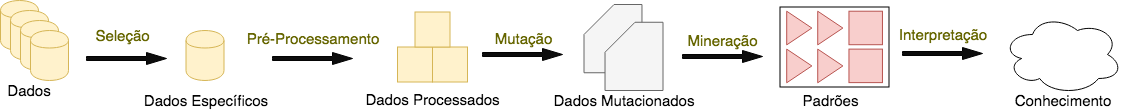
\includegraphics[width=.8\textwidth]{imagens/kdd.png}
    \caption{Representação da metodologia defendida pela KDD. Fonte: o autor.}
    \label{fig:kdd}
\end{figure}

Com o passar do tempo, várias abordagens surgiram para tratar dados e essa massa de pesquisas e definições deu-se por bagunçar em partes as nomenclaturas e definições que estão atrelados a ciência por trás dos dados. Para evitar confusões as definições apresentadas nessa sessão serão sucintas e tem como objetivo futuros tópicos e discussões apresentados durante os resultados dessa pesquisa. Devido a grande divergência, ocorrida pela disseminação rápida de algumas termologias, os termos abordados serão guiados pelas seguintes referencias \cite{laender2002brief, fayyad1996kdd, hand2007principles}.

\subsection{Seleção de Dados}
O ato de selecionar os dados com enfoque no conhecimento que você deseja obter deles afim de gerar um conjunto de dados especifico é também conhecido como \textit{\textbf{data collection}}, durante o processo do KDD é o primeiro passo responsável por gerar um amostra mais focada no problema.

\subsection{Mineração de Dados}
Nessa subseção propõe-se que seja dissertado sobre os processos do KDD a partir da seleção até a interpretação. Vale ressaltar que para obter conhecimento não é necessário uma IA, sistemas de tomada de decisão trabalham com probabilidade matemática sob dados exatos, o que em muitos casos, já seria o suficiente para obter a informação do dado. Entretanto, o foco da pesquisa se baseia na implementação de um sistema inteligente e isso inclina essa explicação para o fato de: o aprendizado de máquina é uma das possíveis formas de se minerar um dado.

A mineração de dados ou popularmente conhecida como \textit{data mining}, baseia-se em retirar os valores mais relevantes e valiosos para se inferir um conhecimento. Os demais passos como pré-processamento e mutação se assemelham a alguns processos citados anteriormente como a redução dimensional ou ainda a engenharia de atributos.


\subsection{Analise de Dados}
E finalmente, a analise. O passo descrito como interpretação no KDD se refere a entender os dados de saída vindos da mineração afim de afirmar ou descarta hipóteses, com isso é possível refinar o processo e explorar novas possibilidades. Uma das palavras que hoje se tornaram popular dentro dá área é o \textit{data storytelling}, ou, o ato do dado de contar uma história. Abordar a hipótese de maneira empírica e demonstrar a veracidade dela discutindo abordagem e algoritmos gerados é um dos objetivos dessa área.


